\section{Makna Geometris Penjumlahan Vektor}

\begin{outcome}

\begin{enumerate}
\item[A.] Memahami penjumlahan vektor secara geometris.
\end{enumerate}
\end{outcome}

Ingat bahwa suatu elemen $\mathbb{R}^{n}$ adalah daftar bilangan yang terurut.
Untuk kasus khusus $n=2,3$, daftar ini dapat digunakan untuk
menentukan sebuah titik dalam ruang dua atau tiga dimensi. Titik ini
ditentukan relatif terhadap beberapa sumbu koordinat.

Perhatikan kasus $n=3$. Ingat bahwa mengambil sebuah vektor lalu memindahkannya
tanpa mengubah panjang atau arahnya tidak mengubah
vektor tersebut. Hal ini penting dalam representasi geometris penjumlahan
vektor.

Misalkan kita memiliki dua vektor, $\vect{u}$ dan $\vect{v}$, dalam
$\mathbb{R}^{3}$. Masing-masing dapat digambarkan secara geometris dengan menempatkan
pangkal setiap vektor di $0$ dan ujungnya masing-masing di $\left( u_{1}, u_{2},
u_{3}\right)$ dan $\left( v_{1}, v_{2}, v_{3}\right) $.
Misalkan kita menggeser vektor $\vect{v}$ sehingga pangkalnya
berada di ujung $\vect{u}$. Kita tahu bahwa tindakan ini tidak mengubah
vektor $\vect{v}$. Sekarang, gambarkan sebuah vektor baru dari pangkal
$\vect{u}$ ke ujung $\vect{v}$. Vektor ini adalah
$\vect{u}+\vect{v}$.

Makna geometris penjumlahan vektor dalam $\mathbb{R}^n$ untuk sebarang $n$ diberikan dalam
definisi berikut.

\begin{definition}{Geometri Penjumlahan Vektor}\label{def:geometryofvectoraddition}
Misalkan $\vect{u}$ dan $\vect{v}$ adalah dua vektor. Geser $\vect{v}$ sehingga
pangkal $\vect{v}$ berada pada ujung $\vect{u}$. Kemudian gambarkan
panah yang bergerak dari pangkal $\vect{u}$ ke ujung $\vect{v}$.
Panah ini merepresentasikan vektor $\vect{u}+\vect{v}$.

\begin{center}
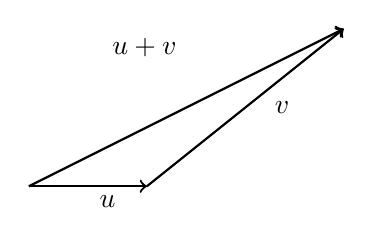
\begin{tikzpicture}[scale=2]
\draw[->, thick](0,0)--(2,1);
\draw[->, thick](0,0)--(0.75,0);
\draw[->, thick](0.75,0)--(2,1);
\node[below left] at (1,1){$\vect{u}+\vect{v}$};
\node[below] at (0.5,0){$\vect{u}$};
\node[right] at (1.5,0.5){$\vect{v}$};
\end{tikzpicture}\par\captionof{figure}{Diagram vektor dua dimensi yang mengilustrasikan aturan ujung-ke-pangkal untuk penjumlahan vektor: panah u di sepanjang...}\label{fig:RnVectorsAdditionMeaning-tikz01}% fig-num-auto

\end{center}
\end{definition}

Definisi ini diilustrasikan dalam gambar berikut, yang menunjukkan
$\vect{u}+\vect{v}$ untuk kasus khusus $n=3$.

\begin{picture}(1,190)
\put(120,40){\begin{picture}(1,1) \thicklines
\setlength{\unitlength}{1pt} \put(0,0){\line(-1,-1){30}}
\put(0,0){\line(0,1){50}}\put(0,0){\line(1,0){80}}
\put(20,80){\put(0,0){\vector(1,1){40}} \qbezier[20](40,40)(40,10)(40,-20)
  \qbezier[10](40,-20)(50,-10)(60,0)
  \qbezier[20](40,-20)(10,-20)(-20,-20)
  \qbezier[10](-20,-20)(-10,-10)(0,0)
  \qbezier[20](0,0)(30,0)(60,0)
  \qbezier[15](0,0)(0,20)(0,40)\put(20,25){$\vect{v}$}}
  \put(0,0){\put(0,0){\vector(1,4){20}}}
  \put(5,50){$\vect{u}$}\put(0,0){\vector(1,2){60}}\put(60,45){$\vect{u}+\vect{v}$}
  \put(55,50){\vector(-1,1){20}}
 \put(0,0){\put(0,0){\vector(1,1){40}} \qbezier[20](40,40)(40,10)(40,-20)
  \qbezier[10](40,-20)(50,-10)(60,0)
  \qbezier[20](40,-20)(10,-20)(-20,-20)
  \qbezier[10](-20,-20)(-10,-10)(0,0)
  \qbezier[20](0,0)(30,0)(60,0)
  \qbezier[15](0,0)(0,20)(0,40)
  \put(22,15){$\vect{v}$}}
  \put(-35,-25){$x$}
  \put(-10,45){$z$}
  \put(75,3){$y$}
  \put(40,40){\qbezier[15](0,0)(10,40)(20,80)}
\end{picture}}
\end{picture}\par\captionof{figure}{Penjumlahan vektor dalam tiga dimensi: u + v sebagai diagonal paralelipiped.}\label{fig:vector-addition-3d}% fig-num-auto


Perhatikan jajargenjang yang dibentuk oleh $\vect{u}$ dan $\vect{v}$ pada diagram di atas.
Maka $\vect{u} + \vect{v}$ adalah diagonal berarah
dari jajargenjang yang ditentukan oleh kedua vektor $\vect{u}$ dan
$\vect{v}$.

Ketika Anda memiliki vektor $\vect{v}$, invers aditifnya $-\vect{v}$ adalah
vektor yang memiliki magnitudo sama dengan $\vect{v}$ tetapi berarah
berlawanan. Ketika seseorang menulis $\vect{u}-\vect{v,}$, artinya adalah $\vect{u} + \left(
-\vect{v}\right) $, seperti halnya pada bilangan real. Contoh berikut mengilustrasikan definisi dan konvensi tersebut.

\begin{example}{Menggambar Penjumlahan Vektor}\label{exa:graphingvectoraddition}
Perhatikan gambar vektor $\vect{u}$ dan $\vect{v}$ berikut.

\begin{center}
\begin{tikzpicture}[scale=2]
\draw[->, thick, blue] (0,0)--(2,1);
\draw[->, thick, red] (4,1)--(5,0.5);
\node[below] at (1,1.25){$\vect{u}$};
\node[above right] at (4.5, 0.75){$\vect{v}$};
\end{tikzpicture}\par\captionof{figure}{Sketsa dua dimensi vektor u (biru, ke atas dan ke kanan) serta v (merah, ke bawah dan ke kanan) yang digambar sebagai...}\label{fig:RnVectorsAdditionMeaning-tikz02}% fig-num-auto

\end{center}

Buatlah sketsa $\vect{u}+\vect{v},\vect{u}-\vect{v}.$
\end{example}

\begin{solution}
Pertama-tama kita akan membuat sketsa $\vect{u}+\vect{v}.$ Mulailah dengan menggambar $\vect{u}$,
lalu, pada ujung $\vect{u}$, tempatkan pangkal $\vect{v}$ seperti
ditunjukkan. Kemudian $\vect{u}+\vect{v}$ adalah vektor yang diperoleh dengan
menggambar sebuah vektor dari pangkal $\vect{u}$ ke ujung $\vect{v}$.

\begin{center}
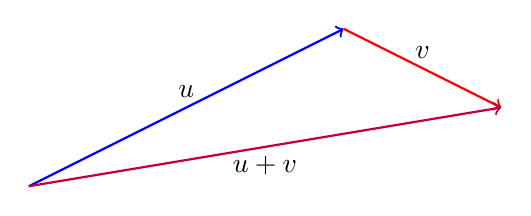
\begin{tikzpicture}[scale=2]
\draw[->, thick, blue](0,0)--(2,1);
\draw[->, thick, red](2,1)--(3,0.5);
\draw[->, thick, purple](0,0)--(3,0.5);
\node[above] at (1,0.5){$\vect{u}$};
\node[above] at (2.5, 0.75){$\vect{v}$};
\node[below] at (1.5, 0.25){$\vect{u}+\vect{v}$};
\end{tikzpicture}\par\captionof{figure}{Diagram vektor dua dimensi u+v yang digambar dengan aturan ujung-ke-pangkal: u berwarna biru dari titik asal ke kanan atas...}\label{fig:RnVectorsAdditionMeaning-tikz03}% fig-num-auto

\end{center}

Berikutnya, perhatikan $\vect{u}-\vect{v}.$ Ini berarti $\vect{u}+\left( -\vect{v}
\right) .$ Berdasarkan uraian geometris penjumlahan vektor di atas, $-\vect{v}$
adalah vektor yang memiliki panjang sama tetapi menunjuk ke arah
yang berlawanan dengan $\vect{v}$. Berikut gambarnya.

\begin{center}
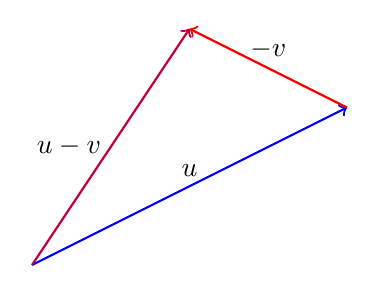
\begin{tikzpicture}[scale=2]
\draw[->, thick, blue](0,0)--(2,1);
\draw[->, thick, red](2,1)--(1,1.5);
\draw[->, thick, purple](0,0)--(1,1.5);
\node[above] at (1,0.5){$\vect{u}$};
\node[above] at (1.5, 1.25){$-\vect{v}$};
\node[left] at (0.5, 0.75){$\vect{u}-\vect{v}$};
\end{tikzpicture}\par\captionof{figure}{Diagram vektor dua dimensi u-v: u berwarna biru dari titik asal, -v berwarna merah yang berawal di ujung u dan...}\label{fig:RnVectorsAdditionMeaning-tikz04}% fig-num-auto

\end{center}
\end{solution}
